%Midterm exam for CS461 for Fall 2003

\documentclass[11pt]{article}
\usepackage{fullpage,pst-all,epsfig}

\newcommand{\comment}[1]{}
\newcommand{\Le}{\textbf{L}}

\newcommand{\ans}[1]{\emph{Solution: #1}}
%\newcommand{\ans}[1]{ }

\newcommand{\seq}[1]{ \langle #1,\cdots \, \rangle}
\newcommand{\seqi}[1]{ \langle #1 \rangle}
	
\begin{document}
\thispagestyle{empty}
\begin{center}
\def\handout{Final Examination}
\vspace*{-.75in}
{\large University of New Mexico}\\
{\large Department of Computer Science}\\
\vspace*{0.5in}
{\LARGE {\bf \handout}}\\
\vspace*{0.1in}
{\large CS 561 Data Structures and Algorithms}\\
{\large Fall, 2010}\\ [0.3in]
\end{center}

\vfill

\makeatletter
\long\def\hint#1{({\em Hint\/}: #1)}
% \def\@oddhead{\rm\makebox[0in][l]{CS 461 Midterm ---Fall,
% 2003}\hfil\thepage\hfil\makebox[0in][r]{Name:\rule[-0.1in]{2in}{.5pt}}}
\let\@evenhead\@oddhead
\def\@oddfoot{}
\let\@evenfoot\@oddfoot

\def\problem#1{\def\problemheading{#1}\clearpage\item{\bf #1}}

% Comment out the above 'problem' def and use the one below to get
% all the problems on a single page, instead of page break each time.
%\def\problem#1{\def\problemheading{#1}\item{\bf #1}}

\def\extrapage{\addtocounter{enumi}{-1}\clearpage\item{\bf \problemheading, continued.}}

\let\part\item
\renewcommand{\theenumii}{\alph{enumii}}
\makeatother
\parindent 0pt

\vfill
\centerline{
\Large
\begin{tabular}{|l|}  \hline
Name: \hspace*{2in} \\ \hline
Email: \hspace*{2in}\\ \hline
\end{tabular}
}
\vfill

\hrule
\begin{itemize}

\item ``Nothing is true.  All is permitted'' - Friedrich Nietzsche.  Well, not exactly.  \emph{You are not permitted to discuss this exam with any other person.}  If you do so, you will surely be smitten.  You may consult any \emph{other} sources including books, papers, web pages, computational devices, animal entrails, seraphim, cherubim, etc. in your quest for truth and solutions.  Please acknowledge your sources.

\item {\em Show your work!}  You will not get full credit if we cannot figure out how you arrived at your answer.  A numerical solution obtained via a computer program is unlikely to get much credit, if any, without a correct mathematical derivation.

\item Write your solution in the space provided for the corresponding problem.

\item If any question is unclear, ask for clarification.

\end{itemize}
\hrule
\vfill
\centerline{
\Large
\begin{tabular}{|c|c|c|c|}  \hline
Question & Points & Score & Grader \\  \hline\hline
1 & 10 & & \\  \hline
2 & 10 & & \\  \hline
3 & 20 & & \\  \hline
4 & 20 & & \\  \hline
5 & 20 & & \\  \hline
6 & 20 & & \\  \hline
7 & 30 & & \\  \hline
\hline Total & 130 & & \\  \hline
\end{tabular}
}
\vfill

\newpage

 
 \begin{enumerate}
 
 \problem{Spanning Trees}
 
 \begin{enumerate}
 \item (5 points) Prove that in a graph where all edge weights are the same, that any breadth first search tree will also be a minimum spanning tree.
 
\ans{In such a graph, any spanning tree is also a MST since any spanning tree contains exactly $n-1$ edges} \ \\ \ \\ \ \\ \ \\ \ \\ \ \\ \ \\ \ \\ \ \\ \ \\
   
 \item (5 points) Consider an undirected graph where every edge has a unique positive weight.  Is it the case that the shortest path tree rooted at $v$ on that graph is always the same as the minimum spanning tree found by Prim's algorithm when seeded initially with the vertex $v$.  If so, prove it.  If not, give a counter example.

\ans{No.  Consider the graph over vertices $v,w,x$ where edge $(v,w)$ has weight $1$, edge $(v,x)$ has weight $2.5$ and edge $(w,x)$ has weight $2$.  The shortest path tree for $v$ is edges $(v,w)$ and $(v,x)$.  The MST found by Prim's when started at $v$ is $(v,x)$ and $(w,x)$.}
\end{enumerate}

 
 
 
 \problem{Donuts}
A certain bakery sells donuts in boxes of three different quantities, $x_{1}$, $x_{2}$, and $x_{3}$. In the Donut
Buying problem, you are given the numbers $x_{1}$, $x_{2}$ and $x_{3}$, and an integer $n$ and you should return either 1) the minimum number of boxes needed to obtain exactly $n$ donuts if this is possible, along with a set of boxes that obtains this minimum; or 2) ``DOH!'' if it is not possible to obtain exactly $n$ donuts.  

For example if $x_{1} = 4$, $x_{2} = 6$, $x_{3} = 9$ and $n = 17$, then you should return that $3$ boxes suffices, with $2$ boxes of size $4$, and $1$ box of size $9$.
However, if $n = 11$, you should return �DOH!� since it is not possible to buy exactly $11$ donuts with these box sizes.

\begin{enumerate}

\item (5 points) For any positive $x$, let $m(x)$ be the minimum number of boxes needed to buy $x$ donuts if this is possible, or INFINITY otherwise.  Write a recurrence relation for the value of $m(x)$.  Don't forget the base case(s)!

\ans{$m(0) = 0$ and for all $x<0$, $m(x)$ is infinity.  For $x>0$, $m(x)$ is $1 + $ the minimum of $m(x-x_{1})$, $m(x-x_{2})$, $m(x-x_{3})$.} \\ \ \ \ \\ \ \\ \ \\ \ \ \ \\



\item (5 points) Give an efficient algorithm for solving Donut Buying. How does its running time depend on $x_{1}$, $x_{2}$, $x_{3}$,
and $n$? Is it an algorithm that runs in polynomial time in the input sizes?  

\ans{This is just a dynamic program where we store the $m$ values in an array of size $n$, where we fill in values left to right.  We also store back edges to keep track of which box was used to obtain each minimum value.  If $m(n)$ is infinity, we return ``DOH''.  Otherwise, we follow the edges back to obtain the boxes need in the optimal solution.  The algorithm does NOT run in polynomial time in the inputs since $n$ is represented with $\log n$ bits only.  Thus, it is an exponential time algorithm.}

 \end{enumerate}
 
 
 \problem{Amortized Analysis}
(20 points) Consider a new data structure that combines the properties of both stacks and queues.  It may be viewed as a list of elements written left to right with three possible operations:
\begin{itemize}
\item Push: add a new item to the left end of the list
\item Pop: remove the item on the left end of the list
\item Pull: remove the item on the right end of the list
\end{itemize}

Show how to implement this new data structure using only: one stack, one queue, and $O(1)$ additional memory, so that the amortized time for all three operations is $O(1)$.  {\bf You are allowed to access the  stack and queue only through the standard PUSH, POP and PULL operations}.  Don't forget to prove your operations have $O(1)$ amortized cost.

\ans{Call the new data structure a quack and let S be the stack and Q be the queue.  We will keep track of the value n, which is the number of items on the quack, i.e. the max of $0$ and the number of times push has been called minus the number of times Pop or Pull have been called.  When an item is pushed onto the quack, push it onto both S and Q.  If $n>0$, then when an item is popped from the quack, call POP on S and when an item is pulled from the quack, call PULL from Q.  However, if $n=0$, when either pop or pull is called on the quack, do 1) call POP on S until it is empty; 2) call PULL on Q until it is empty; and 3) return ``ERROR: Empty Quack''.  We can use the accounting method to show the amortized run time.  Charge \$3's for each call to Push and \$0's for the other operations.  When an item $x$ is pushed on the Quack, store one dollar with the item that is pushed on $S$ and one dollar with the copy pushed on $Q$.  When calling POP or PULL on S or Q, each item will have a dollar on it to pay for the time for removal!}
 
 
\problem{Commodities Trading} 
 (20 points) Imagine there are $n$ commodities $g_{1}, g_{2}, \ldots, g_{n}$ and an $n$ by $n$ table $R$ of exchange rates, such that one unit of commodity $g_{i}$ can be traded for $R[i,j]$ units of commodity $j$.  Moreover, there are \emph{taxes} on each commodity given by $t_{1}, t_{2}, ..., t_{n}$ such that if $i$ is an intermediate commodity in a sequence of trades, you are taxed at rate $t_{i}$ when you convert to commodity $i$.  For example, when you convert to the intermediate commodity ``pork bellies'', you are taxed at a rate of $.05$.  A \emph{valid} sequence of trades, starts and ends with the same commodity.  The \emph{revenue} from a sequence of trades is the amount of the first commodity you end up with if you start with one unit of the first commodity initially and perform the trades in the sequence.  For example, if there is a sequence of commodities $g_{i_{1}}, g_{i_{2}}, \ldots, g_{i_{k}}, g_{i_{1}}$, then the profit for that sequence is: $R[i_{1}, i_{2}] \cdot (1 - t_{2}) \cdot R[i_{2}, i_{3}] \cdot(1 -  t_{3}) \cdots R[i_{k-1},i_{k}] \cdot (1- t_{k}) \cdot R[i_{k},i_{1}] \cdot (1-t_{1})$.  Note that you are only taxed once for the start/end commodity in the valid sequence.  Note also that the revenue may be less than $1$.

Your goal is to design an algorithm that finds some valid sequence of trades with revenue greater than $1$ if such a sequence exists, or outputs NONE if no such sequence exists.  Show how to do this using techniques from class.  Don't forget to analyze the runtime of your algorithm.

\ans{Create a graph, $G$, with source vertex $s$, and for each commodity $v$, there is a vertex $v_{i}$ and $v_{o}$.  For each commodity $v$, add edge from $s$ to $v$ with weight $0$; and also add an edge from $v_{i}$ to $v_{0}$ with weight $- \log (1-t_{v})$.  Finally, for each commodity $u$ and $v$, add an edge from $u_{o}$ to $u_{i}$ with weight $- \log R[u,v]$.  Now run Floyd Warshall to determine if there is a negative cycle in $G$.  The runtime is dominated by the runtime of Floyd Warshall, which is $O(n^{3})$.}

 

\problem{Dinner Party} 
(20 points) You are giving a large dinner party. There are $n$ guests who you will have to split up over
two  tables. Assume that for any two people, $i$ and $j$, there is a nonnegative cost $c_{i,j}$ if they
sit at different tables. Moreover, each person has given you information about their table preferences: for each $i$ there is a nonnegative cost $a_{i}$
if they do not sit at table A, and a nonnegative cost $b_{i}$ if they do not sit at table B. Your goal is to divide the guests into two sets A and B, seating them at the
corresponding tables, in a way that minimizes the total cost:
$ \sum_{i \in A} b_{i} + \sum_{i \in B} a_{i} + \sum_{(i,j): i \in A \textrm{ and } j \in B} c_{i,j}$

Give an efficient algorithm to solve this problem based on min-cuts.  Argue that your algorithm is correct and analyze its runtime.
 
\ans{This is a min-cut problem.  We create a new network $G$, with a node for each of the people in the network and additional nodes $s$ and $t$.  We create edges from every node $s$ and every node associated with each person $i$ to $s$ with edge weight $a_{i}$.  We also create edges from each person $i$ to $t$ with edge weight $b_{i}$.  Finally, for every person $i$ and every person $j$, we create an edge from node $i$ to node $j$ with weight $c_{i,j}$.  Now we find the minimum $s$, $t$ cut in this network.  Intuitively, the $s$ side of the cut will represent everyone sitting at table A and the $t$ side will represent everyone sitting at table B.  You can use the Dinits algorithm to find the min cut in this network for a total runtime of $O(nm^{2})$ which is $O(n^{5})$ in this case.} 
 
 
 
 \problem{Rock, Paper, Scissors}
 
 Rock, Paper, Scissors is a simple 2 person game.  In a given round, both players simultaneously choose either Rock, Paper or Scissors.  If they both choose the same object, it's a tie.  Otherwise, Rock beats Scissors; Scissors beats Paper; and Paper beats Rock.  Imagine you're playing the following betting variant of this game with a friend.  When Scissors beats Paper, or Paper beats Rock, the loser gives the winner
 \$1.  However, in the case when Rock beats Scissors, this is called a SMASH, and the loser must give the winner \$10.  
 
 
 \begin{enumerate}
 \item (6 points) Say you know that your friend will choose Rock, Scissors or Paper, each with probability $1/3$.  Write a linear program to calculate the probabilities you should use of choosing each object in order to maximize your expected winnings.  Let $p_{1}, p_{2}, p_{3}$ be variables associated with the best way of choosing Rock, Scissors and Paper respectively.  Note: If you want to check your work, there are several free linear program solvers on the Internets: check the Wikipedea page on linear programming.
 
 \ans{Let $p_{1}, p_{2}, p_{3}$ be variables associated with you choosing Rock, Scissors and Paper respectively.\\ Maximize: $10*(1/3)*p_{1} - 1*(1/3)*p_{1} - 10*(1/3)*p_{2} + 1*(1/3)*p_{2} +  1*(1/3)*p_{3} - 1*(1/3)*p_{3}$ \\ Subject to the following constraints: \\ $0 \leq p_{1} \leq 1$, $0 \leq p_{2} \leq 1$, $0 \leq p_{3} \leq 1$\\ $p_{1} + p_{2} + p_{3} = 1$}
 
 \pagebreak

 
 \item (14 points) Now say that your friend is smart and, also, clairvoyant: she will magically know the exact probabilities you are using and will respond optimally.  Write another linear program to calculate the probabilities you should now use in order to maximize your expected winnings.  Hint 1: If your opponent knows your strategy, her strategy will be to choose one of the three objects with probability $1$.  Hint 2: Review the LP for shortest paths in the last HW.
 
\ans{
Let $p_{1}, p_{2}, p_{3}$ be variables associated with you choosing Rock, Scissors and Paper respectively.
Maximize: $w$\\
Subject to:\\
$0 \leq p_{1} \leq 1$, $0 \leq p_{2} \leq 1$, $0 \leq p_{3} \leq 1$\\ $p_{1} + p_{2} + p_{3} = 1$
$ w \leq 1*p_{3} -10 * p_{2}$ - opponent always chooses rock\\
$ w \leq 10*p_{1} - 1*p_{3}$ - opponent always chooses scissors\\
$ w \leq 1*p_{2} - 1*p_{1}$ - opponent always chooses paper\\
}


 \end{enumerate}
 
 
 

 
 
 
 \problem{File Movement}
 
 In the File Movement problem, you want to move files from an initial configuration to a goal configuration in a network of $n$ completely connected computers, as quickly as possible.  The files are all of equal size, and in any one round, a computer can be involved in either sending a file or receiving a file, {\bf but not both} \footnote{The files are so large that they must be read or written to disk directly.  Thus, either sending or receiving a file requires complete control of the disk.}.  You've decided that you can recast this problem as a problem in graph theory as follows.  You  are given a graph $G=(V,E)$, where $V$ is the set of all computers, and there is an edge from $x$ to $y$ in $E$ for each file that starts at $x$ and wants to go to $y$.  {\bf Note that there may be multiple edges in $G$ from $x$ to $y$ if multiple files want to move from $x$ to $y$.}  Your goal is to label each edge in $G$ with a positive integer such that: 1) for every node $v$ in $G$, all edges touching $v$ have unique numbers; and 2) the largest integer used is as small as possible.  
 
See the figure below for an example.
 
 \begin{figure}[htbp]
\begin{center}
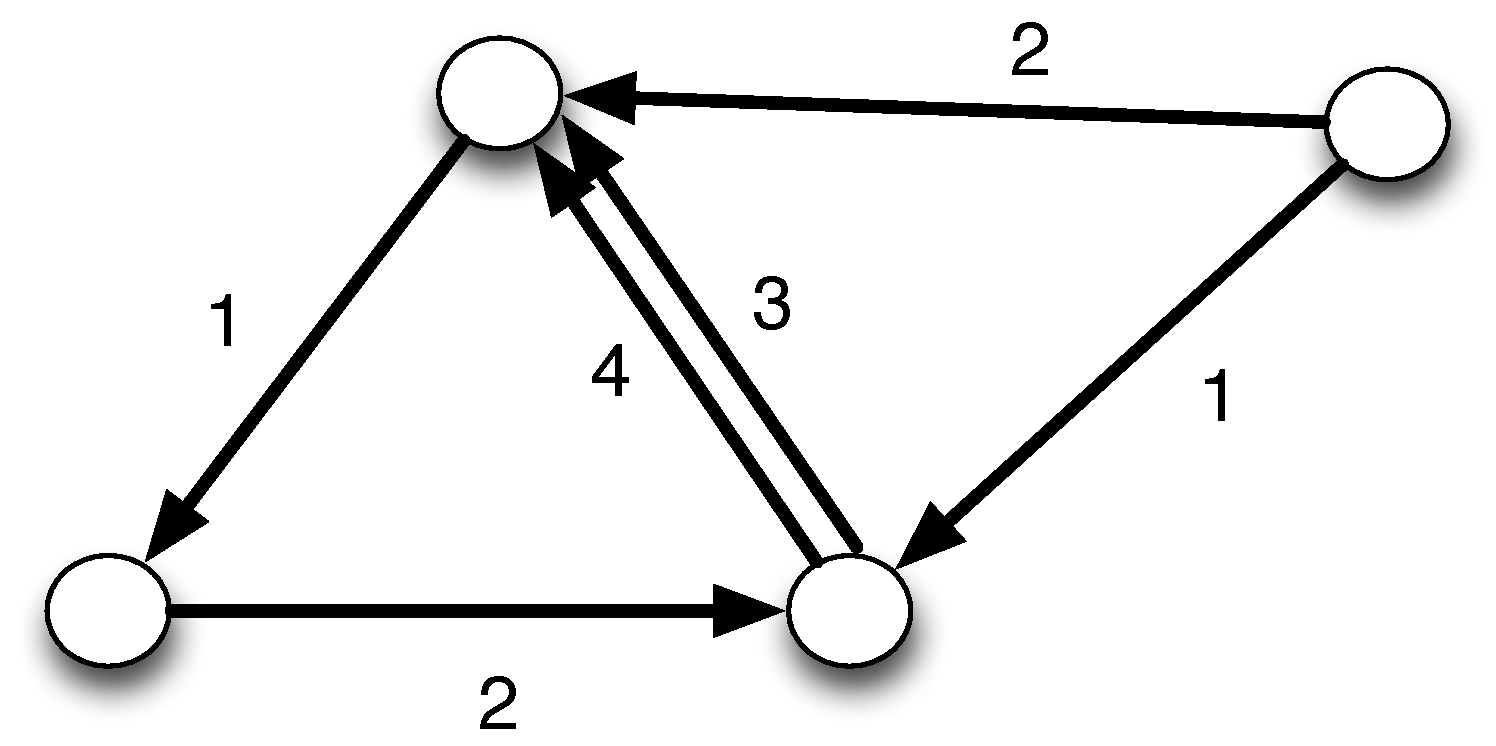
\includegraphics[scale=0.23]{file-moving.pdf}
\caption{File Movement problem with $4$ computers and $6$ files.  The labeling shows that all files can be moved in $4$ rounds.}
\label{default}
\end{center}
\end{figure}

 
 \begin{enumerate}
 
 \item (10 points) Assume you are given a directed graph $G$ where every vertex has out-degree $k$ and in-degree $k$, for some value $k \geq 2$.  Describe an algorithm, based on techniques from this class, that gives a valid labeling for $G$, and that uses no more than $3k$ different numbers.  Show that your algorithm is correct and analyze its runtime when $n$ is the number of vertices in $G$.  Hint 1:  Repeatedly find a collection of cycles such that every vertex in the graph appears exactly once, in exactly one cycle in the collection.  Hint 2: bipartite matching.

\ans{Set up bipartite graph with all nodes in $G$ on left side and copies of all nodes on right.  Edges in this graph are edges from $G$, all going from left to right.  Because the graph is $k$ regular, Hall's Theorem applies.  Why?  We can thus find a perfect matching using network flow and this matching will induce the collection of cycles desired.  We can label each collection of cycles with at most $3$ different colors (all even cycles need only $2$ colors, and odd cycles require only $3$).  The total number of collections of cycles will be exactly $k$.  Thus we will require exactly $3k$ different colors.}

\extrapage

\item (10 points) Now assume that you are given directed graph $G$ over $n$ vertices, and also have an additional $n/3$ free ``helper'' computers.  Show how you can use these helper computers to get a labeling that requires only $2k$ numbers.


\ans{Obtain the decomposition into cycles as above.  Then simply insert one of the helper machines into each odd cycle that occurs in a collection, in order to make that cycle even, and to allow a labeling with just $2$ numbers.  There are at most $n/3$ odd cycles, so $n/3$ helper computers suffice.}


\pagebreak

\item (10 points) {\bf (Challenge)} Now what if the maximum degree of $G$ is $K$, but $G$ is not necessarily regular.  Describe an efficient algorithm to find a labeling that uses at most $\lceil(3/2)K \rceil$ numbers without any helper computers, and at most $K+1$ number with $n/3$ helpers.  Hint: Google ``Eulerian Cycle''.  Assume you have an efficient algorithm to solve Eulerian Cycle.

\ans{Add enough dummy edges to $G$ to ensure that the degree of each node is exactly  $2 \lceil K/2 \rceil$.  (How?  See me if you need help on this.)  Now find an Eulerian cycle on this new graph and orient each edge based on the direction it is traversed in the Eulerian Cycle.   At this point, the graph will have degree $\lceil(3/2)K \rceil$, and will have the same form as the graph described in parts a) and b)}





\end{enumerate}


 
\end{enumerate}
\end{document}


\problem{Shortest Paths, Commodities and the Moral Torpidity of American Enterprise}
 
 \emph{``A million dollars isn't cool.  You know what's cool?  A billion dollars'' - Sean Parker in The Social Network}
 
What if we change the all-pairs, shortest paths problem so there is some cost associated with each intermediate vertex that is traversed in a path?  In particular, we are given a graph $G$ that has weights, $w$, on all the edges and also weights, $w'$, on all the vertices.  The weight of a path is the sum of the weights of all edges in that path and the weights of all vertices in the path except for the start and end vertex.  For example, the weight of the path $v_{1}, v_{2}, v_{3}, v_{4}$ is $w(v_{1} \rightarrow v_{2}) + w(v_{2} \rightarrow v_{3}) + w(v_{3} \rightarrow v_{4}) + w'(2) + w'(3)$.  The weights of both edges and vertices may be negative.  Your first goal is to design an algorithm that either computes the weight of the shortest path between every pair of vertices if there is no negative weight cycle in the graph, or else if there is a negative weight cycle, correctly returns that this is the case.

You will show how to modify the Floyd Warshall algorithm to solve this new variant of all pairs shortest paths.  As in lecture, let $dist(u,v,r)$ be the shortest path from $u$ to $v$ that traverses vertices numbered $r$ or less.  Also, assume that the vertices are uniquely labelled from $1$ to $n$

\begin{enumerate}
\item (8 points) Write down a recurrence relation for $dist(u,v,r)$ for this new variant of the shortest paths problem. 

\ans{$dist(u,v,r) = w(u \rightarrow v)$ if $r=0$\\ else $dist(u,v,r) = min (dist(u,v,r-1), dist(u,r,r-1) + dist(r,v,r-1) + w'(r)$)}  \ \\ \ \\ \ \\ 

\pagebreak

\item (7 points) Write down an algorithm, based on Floyd Warshall that solves this variant of the shortest path problem.  Remember your algorithm should return that there is a negative weight cycle if one exists.

\ans{Run the lecture notes Floyd Warshall with the above recurrence.  Then at the end, check $dist(u,u,n)$ for all nodes $u$, if any of these values are negative, output that there is a negative weight cycle.}


\pagebreak

\item (10 points) Now imagine that you're trying to make money in the following variant of the arbitrage problem.  There are $n$ commodities $g_{1}, g_{2}, \ldots, g_{n}$ and an n by n table $R$ of exchange rates, such that one one unit of commodity $g_{i}$ buys $R[i,j]$ units of commodity $j$.  Moreover, there are \emph{taxes} on each commodity given by $t_{1}, t_{2}, ..., t_{n}$ such that if $i$ is an intermediate commodity in a sequence of trades, you are taxed at rate $t_{i}$ when you convert to commodity $i$.  For example, when you convert to the intermediate commodity ``pork bellies'', you are taxed at a rate of $.05$.  A \emph{valid} sequence of trades, starts and ends with the same commodity.  The \emph{revenue} from a sequence of trades is the amount of the first commodity you are left with if you start with one unit of the first commodity initially and perform the trades in the sequence.  For example, if there is a sequence of commodities $g_{i_{1}}, g_{i_{2}}, \ldots, g_{i_{k}}, g_{i_{1}}$, then the profit for that sequence is\\ $R[i_{1},i_{2}]\cdot (1 - t_{2}) \cdot R[i_{2}, i_{3}] \cdot(1 -  t_{3}) \cdots R[i_{k-1},i_{k}] \cdot (1- t_{k}) \cdot R[i_{k},i_{1}]$

(Note that you are never taxed for the start/end commodity in the valid sequence, and that the revenue may be less than $1$.)

Design an algorithm that either 1) finds some valid sequence of trades with revenue greater than $1$ and outputs this revenue; or 2) if there is no valid sequence with revenue greater than $1$, outputs the maximum revenue possible from a valid sequence of trades.

\ans{Create a graph with a vertex for every commodity.  Let the weight of edge $u \rightarrow v$ equal $- \log R[u,v]$.  Let the weight of vertex $v$ equal $- \log (1-t_{v})$.  Now run modified Floyd Warshall with the recurrence in the previous problem to fill in all entries of the array.  Find the vertex $v$ that minimizes $dist(v,v,n)$; return $2^{-dist(v,v,n)}$}


\end{enumerate}

 with $4$ machines and $6$ files, along with a labeling showing they can all be moved in $4$ rounds.


\problem{Probability}
 
Have a n by n grid and put m sensors down on it.  Each sensor's broadcast radius is a ball of radius k.  Question:  What is expected number of collisions.  What is bound on probability that no two sensors collide.
 



